\documentclass[12pt,a4paper]{report}
\usepackage[margin=2.50cm]{geometry}
\usepackage{hyperref}
\usepackage[T1]{fontenc}
\usepackage{color}
\usepackage{fancyhdr}
\usepackage[titles]{tocloft}
\usepackage{setspace}
\usepackage{array}
\hypersetup{colorlinks=true, linkcolor=blue, urlcolor=cyan}
\usepackage[pdftex]{graphicx}
\usepackage[parfill]{parskip}
\usepackage{longtable}
\usepackage{float}
\usepackage[english]{babel}

%----------Config Data format---------------------------------------------
\usepackage{datetime}
\newdateformat{dashdate}{\THEYEAR-\twodigit{\THEMONTH}-\twodigit{\THEDAY}}
%-------------------------------------------------------------------------

\begin{document}
%\raggedright{} %Left justified, make report more readable
\pagenumbering{roman}

%----------------------------Cover Page---------------------------------------
\title{This is report title}
\author{Author Name}
\date{today}
\maketitle

%--------------------------Revision History-----------------------------------
\renewcommand*\thesection{\Large{\arabic{section}}}
%\renewcommand*\thesubsection{\Large{\arabic{section. subsection}}}
\section*{Revision History}
	\begin{table}[h!]
		\centering
		\begin{longtable}{|c|c|c|p{7cm}|} \hline
%			\rowcolor[rgb]{0.4,0.8,0.9}  
			\textbf{Version} & \textbf{Date} & \textbf{Reviewer} & \textbf{Brief Details} \\\hline
			\endhead
			\endfoot
			\endlastfoot
			& & & \\\hline
			& & & \\\hline
			& & & \\\hline
			& & & \\\hline
			& & & \\\hline
			& & & \\\hline
			& & & \\\hline
			& & & \\\hline
			& & & \\\hline
			& & & \\\hline
			& & & \\\hline
			& & & \\\hline
			& & & \\\hline
			& & & \\\hline
			& & & \\\hline
		\end{longtable}
		%\caption{Revision History}
	\end{table}
\pagebreak

%----------------------------Executive Summary-----------------------------
\renewcommand{\abstractname}{Executive Summary}
\begin{abstract}
This is pdfLatex template report. When I doing a project, Swinburne University require all student use to write report. This is our team need save all of documentation and code in Swinburne's SVN repository. plain-text can be tracked. The Word cannot be tracked, due to binary file. In this team-based project, my role is documentation manager. I focused on the make document satisfied requirements. Latex is new skills for everyone, so I spend a lost of time to research LaTex and LaTex training. In this template, the distribution of LaTex is pdfLaTex. As a Academic Project team, we are require to submit a pdf version of documents to University,client and supervisor. During writing document, our team use TexStudio. This is a cross-platform editor based on Qt.

\end{abstract}

%----------------------------TABLE OF CONTENTS---------------------------------
\thispagestyle{empty}
\renewcommand\contentsname{Table of Contents}\tableofcontents
\listoffigures
\pagebreak

%----------------Footer/Header FOR REST OF DOCUMENT------------------------
\pagestyle{fancy}
\lhead{University}
\lfoot{Report Name}
\cfoot{\thepage}
\rfoot{Author Name}
\renewcommand{\headrulewidth}{0.4pt}
\renewcommand{\footrulewidth}{0.4pt}

%----------------Body of Document------------------------
\pagenumbering{arabic}

\section{Introduction}

\subsection{Purpose}

\subsection{Background}

\subsection{Scope}

	\begin{figure}[h!]
		\centering
		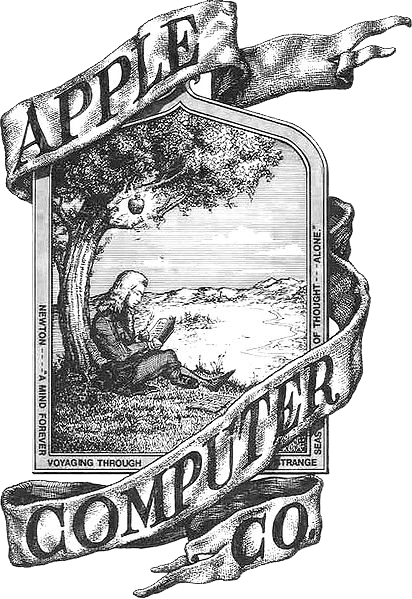
\includegraphics[width=0.5\textwidth]{Apple_first_logo.png}
		\caption{Apple First Logo}
	\end{figure}
	
\section{Body}

\section{Conclusion}

\end{document}
